\documentclass[11pt]{article}
\usepackage[margin=1in]{geometry}
\usepackage{amsmath,amsthm,amssymb}
\usepackage{enumitem, graphicx, float, caption}
\usepackage{amsmath}
\usepackage{bm}
\usepackage{parskip}
\usepackage{lipsum}
\usepackage{tikz}
\usepackage{listings}
\usepackage{xcolor}
\usepackage{subcaption}
\usepackage[utf8]{inputenc}
\usetikzlibrary{arrows.meta}

\definecolor{codegreen}{rgb}{0,0.6,0}
\definecolor{codegray}{rgb}{0.5,0.5,0.5}
\definecolor{codepurple}{rgb}{0.58,0,0.82}
\definecolor{backcolour}{rgb}{0.95,0.95,0.92}

\lstdefinestyle{mystyle}{
    backgroundcolor=\color{backcolour},
    commentstyle=\color{codegreen},
    keywordstyle=\color{magenta},
    numberstyle=\tiny\color{codegray},
    stringstyle=\color{codepurple},
    basicstyle=\ttfamily\tiny,
    breakatwhitespace=false,
    breaklines=true,
    captionpos=b,
    keepspaces=true,
    numbers=left,
    numbersep=5pt,
    showspaces=false,
    showstringspaces=false,
    showtabs=false,
    tabsize=2
}

\lstset{xleftmargin=.13\textwidth, xrightmargin=.10\textwidth}

\setcounter{MaxMatrixCols}{26}
\setlength\parindent{0pt}
\counterwithin{equation}{enumi}


\begin{document}
    \noindent Nathan Burwig \\
    Math 87 HW 4 \\
    Due 10/7/2022
    
    \hrulefill
    
    \begin{enumerate}
        \item Compute the max possible flow from source (node 0) to sink (node
            5) for the following graph. Also, identify the minimum cut.

        \medskip \medskip
        \begin{center}
            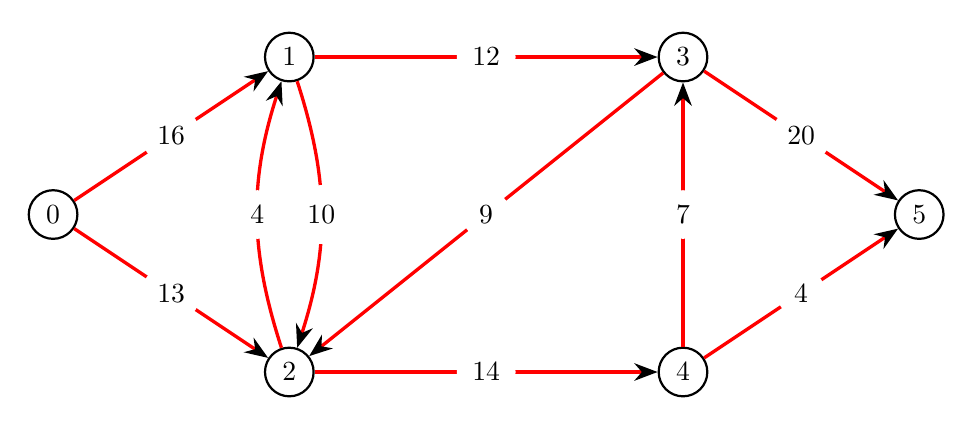
\begin{tikzpicture}
                \begin{scope}[every node/.style = {circle, thick, draw}]
                    \node (A) at (0, 1)    {0};
                    \node (B) at (3, 3)    {1};
                    \node (C) at (3,-1)    {2};
                    \node (D) at (8, 3)    {3};
                    \node (E) at (8,-1)    {4};
                    \node (F) at (11,1)    {5};
                \end{scope}

                \begin{scope}[>={Stealth[black]},
                                every node/.style={fill=white,circle},
                                every edge/.style={draw=red,very thick}]
                    \path [->] (A) edge node {16} (B);
                    \path [->] (A) edge node {13} (C);
                    \path [->] (B) edge[bend left=18] node {10} (C);
                    \path [->] (C) edge[bend left=18] node {4}  (B);
                    \path [->] (B) edge node {12} (D);
                    \path [->] (C) edge node {14} (E);
                    \path [->] (D) edge node {9}  (C);
                    \path [->] (E) edge node {7}  (D);
                    \path [->] (D) edge node {20} (F);
                    \path [->] (E) edge node {4}  (F);
                    
                \end{scope}
            \end{tikzpicture}
        \end{center}
    \end{enumerate}

    We would like to know the max flow of this diagram from source to terminal
    node. We can start this by naming our edges and equally listing out our
    inequality constraings. These are the values on the edges themselves, and
    will be listed out as the values over the edges being maximum values for
    the edge.

    \begin{minipage}[t]{.22\linewidth}
        \begin{align*}
            e_0 &\leq 16     \\
            e_1 &\leq 13     \\ 
            e_2 &\leq 10     \\
            e_3 &\leq 4      \\
            e_4 &\leq 12     \\
            e_5 &\leq 9      \\
            e_6 &\leq 14     \\
            e_7 &\leq 7      \\
            e_8 &\leq 4      \\
            e_9 &\leq 20     
        \end{align*}
        Inequality constraint
    \end{minipage} \hfill \vline \hfill %
    \begin{minipage}[t]{.74\linewidth}
        We can see the inequality constraints off to the left here, and these
        will be neatly put into a vector called \texttt{b}. We will see
        shortly, that we need to add a few zeroes to that vector when we go to
        take the dual linear program. For now these equality constraints are
        fine.

        \medskip
         
        We also have certain equality constraints that are based on the
        conservation rules of the graph above. We know each node will have
        certain edges going in and certain edges going out. We can write
        conservation equations for them. Notably, we will not be writing
        conservation equations for source or terminal, as they either destroy
        or create values that go over the edges, thus they don't conserve
        values. These conservation equations go as follows:
        \begin{align*}
            1)\;\;\;0 &= e_0 + e_2 - e_3 - e_4  \\
            2)\;\;\;0 &= e_1 - e_2 + e_3 + e_5 - e_6    \\
            3)\;\;\;0 &= e_5 + e_6 + e_8 - e_9  \\
            4)\;\;\;0 &= e_6 - e_7 - e_8        \\
        \end{align*}
    \end{minipage}

    From here, we can begin setting up the A matrix, using our equality
    constraints, as well as our inequality constraints. The equality
    represented by the node conservation rules, and the inequality by the
    inequalities shown in upper left.

    \newpage

    We know our constraints now, and can setup a matrix that looks like the
    following...
    \[
        A=
        \begin{bmatrix}
            I_{10}    \\
            \text{Conservation for node 1}  \\
            \text{Conservation for node 2}  \\
            \text{Conservation for node 3}  \\
            \text{Conservation for node 4}  \\
        \end{bmatrix}
    \]
    Lastly, we need an objective function, which we maximize over. We know that
    the edges connected to the source node, are the only edges that will be
    "producing" whatever items will be traversing these edges. Because of this,
    they are the only edges that will have nonzero values in our objective
    function, as we are optimizing over the paths that come from the source
    node. Thus...
    \[
        c=\begin{bmatrix}\; 1 & 1 & 0 & 0 & 0 & 0 & 0 & 0 & 0 & 0\; \end{bmatrix}
    \]
    We now have all the values required to produce a linear program of the
    primal variety. But, we are going to take this and turn it into a dual
    linear program, as we also want to find the minimal cut. The dual linear
    program will give us both the value of the maximal flow, as well as the
    minimal cut. We know that a dual linear program looks something like the
    following:
    \begin{align*}
       b^T \cdot {y} \rightarrow {max} \\
       A^T y \geq c^T
    \end{align*}
    So, we can now see the general setup and can begin putting this all
    together. 

    Taking the transpose of the large A matrix results in another large matrix
    that I will not be printing the entirety of as it would simply take far too
    long and too much space. I will, however, be showing the code that sets up
    the A matrix, and it's general form becomes the following.
    \[
        \begin{bmatrix}
            I_{10}  &   \text{[Conservation for 1, 2, 3, 4$]^T$}
        \end{bmatrix}
    \]
    And thus our matrix goes from being a 14x10 to at 10x14. We then have that
    times our vector $y$ which has the general form $y=\begin{bmatrix}
    \textbf{d} \\ \textbf{p} \end{bmatrix}$ where $d \in \mathbb{R}^{10}$ and $p
    \in \mathbb{R}^4$ all constrained against $c^T$.

    Right, now we can keep talking setup, or we can go ahead and show some
    results, and a little code to further solidify what is going on here.

    \begin{lstlisting}[style=mystyle, language=Python, gobble=8, 
                      caption=The dual linear program]
        import numpy as np
        from scipy.optimize import linprog
        
        def sbv(index,size):
            return np.array([1.0 if i == index-1 else 0.0 for i in range(size)])

        # constraints | inequality | equality                |
        A = np.block([[ sbv(1,10)  , np.array([ 1, 0, 0, 0]) ],
                      [ sbv(2,10)  , np.array([ 0, 1, 0, 0]) ],
                      [ sbv(3,10)  , np.array([1, -1, 0, 0]) ],
                      [ sbv(4,10)  , np.array([ -1, 1, 0, 0]) ],
                      [ sbv(5,10)  , np.array([ -1, 0, 1, 0]) ],
                      [ sbv(6,10)  , np.array([ 0, 1, -1, 0]) ],
                      [ sbv(7,10)  , np.array([ 0, -1, 0, 1]) ],
                      [ sbv(8,10)  , np.array([ 0, 0, 1, -1]) ],
                      [ sbv(9,10)  , np.array([ 0, 0, 0, -1]) ],
                      [ sbv(10,10) , np.array([ 0, 0, -1, 0]) ]])
        
        c = np.array([1, 1, 0, 0, 0, 0, 0, 0, 0, 0])
        
        b = np.array([16, 13, 10, 4, 12, 9, 14, 7, 4, 20, 0, 0, 0, 0])
        bounds = np.array(10*[(0,None)] +  4*[(None,None)])
        
        
        res = linprog(b, A_ub = (-1)*A, b_ub = (-1)*c, bounds=bounds)
        print(res)
    \end{lstlisting}

    A couple notes about the setup here, is the use of the \texttt{bounds}
    parameter which, frankly is something I didn't know existed until looking
    at the example code. After looking it up, it appears to be the upper and
    lower bounds for each decision variable. 
    
    We can also note that $b^T$ has a couple extra zeros on the end of it,
    which are as they account for the inequality constraints on the nodes,
    which are part of the $\textbf{y}$ vector, represented in the $\textbf{p}$
    half of the vector. 

    Solving this results in the following output.

    \begin{minipage}[t]{.3\linewidth}
    \begin{lstlisting}[basicstyle=\small, gobble=12]
            fun: 23.0
              p_0 	0
              p_1 	0
              p_2 	0
              p_3 	0
              p_4 	1
              p_5 	0
              p_6 	0
              p_7 	1
              p_8 	1
              p_9 	0
              d_10 	1
              d_11 	1
              d_12 	0
              d_13 	1
        \end{lstlisting}
        The output of linprog
    \end{minipage} \hfill \vline \hfill%
    \begin{minipage}[t]{.65\linewidth}
        The variables past $p_9$ are associated with the nodes, so we will 
        simply look at the first ten. These values will lign up exactly with
        the edges in our graph. We know, via the min cut theorem, the 
        values which are equal to one, are associated with the
        edges that are a part of the min cut. Thus, edge $e_4, e_7$ and $e_8$
        are part of the min cut. Thus, the minimal sum of the two groups is the
        optimal value. That optimal value is 23.0 which was found when running
        the linear program.
        
        \medskip

        I will show the graph after making the min cut, down below. We can see
        that this cut does in fact separate the grpah as it creates an
        impassable disconnect between the two sets of nodes.
    \end{minipage}

    \vspace{2cm}

    \begin{center}
        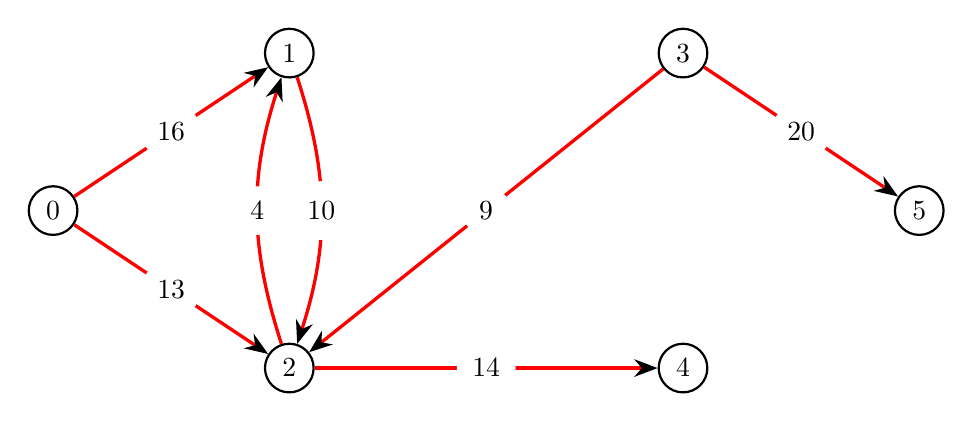
\begin{tikzpicture}
            \begin{scope}[every node/.style = {circle, thick, draw}]
                \node (A) at (0, 1)    {0};
                \node (B) at (3, 3)    {1};
                \node (C) at (3,-1)    {2};
                \node (D) at (8, 3)    {3};
                \node (E) at (8,-1)    {4};
                \node (F) at (11,1)    {5};
            \end{scope}

            \begin{scope}[>={Stealth[black]},
                            every node/.style={fill=white,circle},
                            every edge/.style={draw=red,very thick}]
                \path [->] (A) edge node {16} (B);
                \path [->] (A) edge node {13} (C);
                \path [->] (B) edge[bend left=18] node {10} (C);
                \path [->] (C) edge[bend left=18] node {4}  (B);
                \path [->] (C) edge node {14} (E);
                \path [->] (D) edge node {9}  (C);
                \path [->] (D) edge node {20} (F);
                
            \end{scope}
        \end{tikzpicture}
    \end{center}

 \end{document}
